\documentclass[12pt,a4paper]{article}
\usepackage[utf8]{inputenc}
\usepackage[spanish]{babel}
\usepackage{graphicx}
\usepackage{kpfonts}
\usepackage[left=2cm,right=2cm,top=2cm,bottom=2cm]{geometry}
\begin{document}
\title{Universidad politecnica\\ de la \\ Zona Metropolitana\\ de Guadalajara}
\author{Tarea 3\\ Angel Eraclio Briano Garcia 18311625\\ Ing. Mecatronica 4B}
\maketitle
\begin{figure}[h!]
\centering

\includegraphics[scale=1]{untitled.png} 
\end{figure}
\newpage
\section{Motor de corriente directa}
El motor de corriente continua, denominado también motor de corriente directa, motor CC o motor DC (por las iniciales en inglés direct current), es una máquina que convierte energía eléctrica en mecánica, provocando un movimiento rotatorio, gracias a la acción de un campo magnético.

Un motor de corriente continua se compone, principalmente, de dos partes: - El estátor da soporte mecánico al aparato y contiene los polos de la máquina, que pueden ser o bien devanados de hilo de cobre sobre un núcleo de hierro, o imanes permanentes. - El rotor es generalmente de forma cilíndrica, también devanado y con núcleo, alimentado con corriente directa a través las delgas, que están en contacto alternante con escobillas fijas.

El principal inconveniente de estas máquinas es el mantenimiento costoso y laborioso debido, principalmente, al desgaste que sufren las escobillas al entrar en contacto con las delgas.

Algunas aplicaciones especiales de estos motores son: los motores lineales, cuando ejercen tracción sobre un riel, servomotores y motores paso a paso. Además existen motores de CC sin escobillas (brushless en inglés) utilizados en el aeromodelismo por su bajo par motor y su gran velocidad.

Es posible controlar la velocidad y el par de estos motores utilizando técnicas de control de motores de corriente continua.
\begin{figure}[h!]
\centering
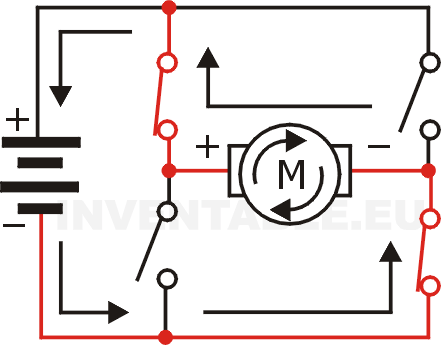
\includegraphics[scale=1]{motor_dc_puente_con_interruptores_giro_orario.png} 

\end{figure}
\newpage
\section{Principio de funcionamiento}
El principio de funcionamiento básico de un motor de CC se explica a partir del caso de una espira de material conductor inmersa en un campo magnético, a la cual se le aplica una diferencia de potencial (o voltaje) entre sus extremos, de forma que a través de la misma circula una corriente I.

Para este caso la espira constituye el rotor del motor, y los imanes que producen el campo magnético constituyen el estátor.

Entonces, dado que cuando un conductor, por el que pasa una corriente eléctrica, se encuentra inmerso en un campo magnético, éste experimenta una fuerza según la Ley de Lorentz. Donde dicha fuerza, denominada Fuerza de Lorentz, es perpendicular al plano formado por el campo magnético y la corriente.
\begin{figure}[h!]
\centering
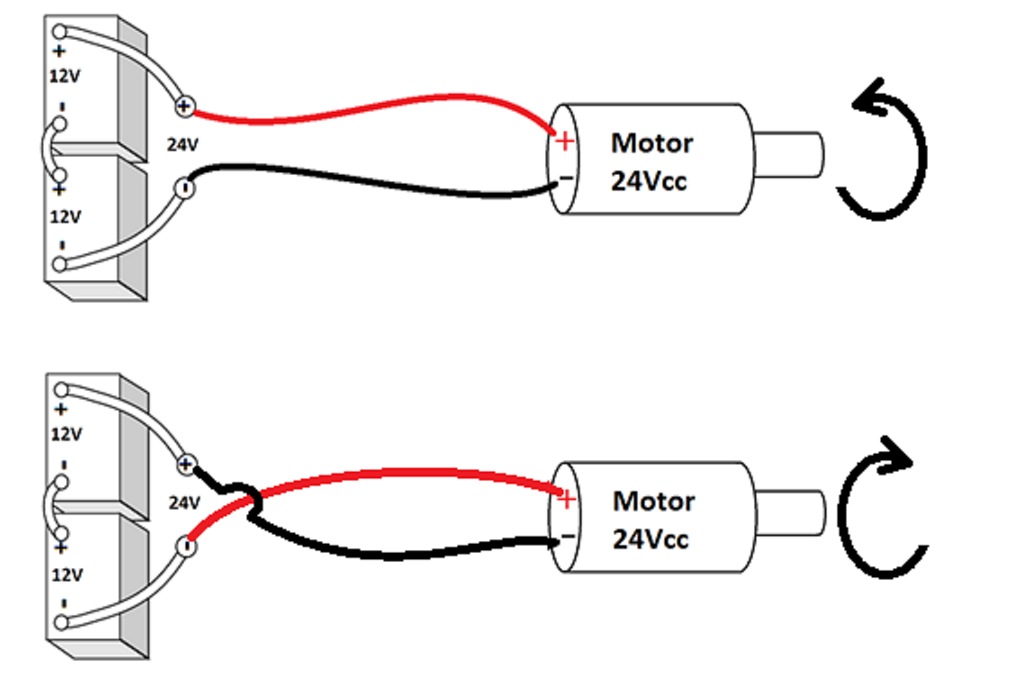
\includegraphics[scale=.5]{conexion motor cc.png} 
\end{figure}
\section{Sentido de giro}
En máquinas de corriente directa de mediana y gran potencia, es común la fabricación de rotores con láminas de acero eléctrico para disminuir las pérdidas asociadas a los campos magnéticos variables, como las corrientes de Foucault y las producidas por histéresis.
\newpage
\section{Reversibilidad}
Los motores y los generadores de corriente continua están constituidos esencialmente por los mismos elementos, diferenciándose únicamente en la forma de utilización. Por reversibilidad entre el motor y el generador se entiende que si se hace girar el rotor, se produce en el devanado inducido una fuerza electromotriz capaz de transformarse en energía eléctrica. En cambio, si se aplica una tensión continua al devanado inducido del generador a través del colector delga, el comportamiento de la máquina ahora es de motor, capaz de transformar la fuerza contraelectromotriz en energía mecánica.

En ambos casos el inducido está sometido a la acción del campo magnético del inductor principal en el estátor.
\begin{figure}[h!]
\centering
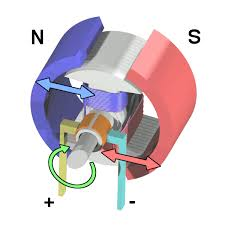
\includegraphics[scale=1]{images.png} 

\end{figure}
\end{document}